\subsection{Dữ liệu: Khung tham chiếu - Không gian}
Tominski và Schulz [415] giới thiệu kĩ thuật trực quan hóa cho dữ liệu thời gian có yếu tố không gian địa lý 2D và thời gian tuyến tính 1D. Ý tưởng là xây dựng một lát cắt không phẳng được gọi là \textit{Great Wall of Space-Time} (hình 7.4) thông qua không-thời gian liên tục 3D (2D+1D). Kiến trúc bức tường này được xây dựng dựa trên các khía cạnh tô tô và hình học của không gian địa lý. Dựa trên một đồ thị lân cận, một đường tô pô được thiết lập tự động hoặc có tương tác. Đường tô pô này được biến đổi thành đường địa lý thông qua những tính chất địa lý của khu vực trên bản đồ. Đường này được dựng thành một bức tường 3D mà chiều thứ 3 có thể được dùng để ánh xạ đến miền thời gian. Những biểu diễn trực quan khác nhau có thể được chiếu lên bức tường này để biểu thị dữ liệu. Bức tường có lợi thế là nó thể hiện một đường khép kín qua không gian mà không có khoảng trống giữa các pixel mang thông tin trên màn hình. 
\begin{figure}[H] % places figure environment here   
    \centering % Centers Graphic
    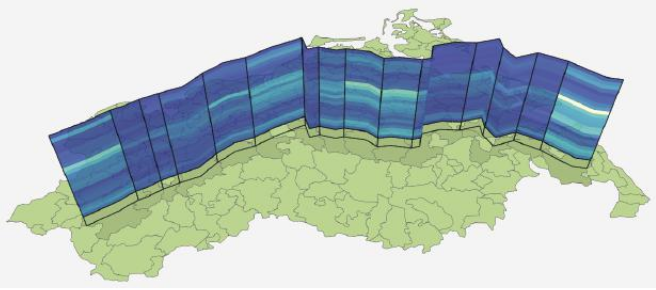
\includegraphics[width=1\textwidth]{assets/fig_7_4.png} 
    \caption{Biểu diễn trực quan hoa của dữ liệu sức khỏe con người sử dụng Great Wall of Space-Time. Một đường trong không gian được thiết lập. Dọc theo đường này, bức tường thể hiện 24 tháng của dữa lioeeuj tại mỗi vùng nó đi qua. Các màu tối thể hiện giá trị dữ liệu thấp, màu sáng thể hiện giá trị cao. Hình trên mô tả số ca mắc cúm } % Creates caption underneath graph
    \label{fig:f7.4}
\end{figure}